% =====================================================================
%  Prabhavit Gupta — one-page CV template (tailor the 3 marked blocks)
%  Compile:  pdflatex -interaction=nonstopmode Prabhavit_CV_TEMPLATE.tex
%  Needs:    photo.jpg  in the same folder as this .tex
%  Rules:    ONE PAGE. No em-dashes. Plain voice. Clickable companies.
%            No "sample of my code" line. Salary blank or "negotiable".
%            Never write "no-code" or "Bubble" — say "off a legacy stack".
% =====================================================================
\documentclass[a4paper,10pt]{article}

\usepackage[T1]{fontenc}
\usepackage[utf8]{inputenc}
% One-page fit lever #1: margins. 0.8cm top/bottom + 1.0cm sides fits ~all content.
\usepackage[top=1.0cm,bottom=1.0cm,left=1.0cm,right=1.0cm]{geometry}
\usepackage{setspace}
\setstretch{1.15}
\usepackage{titlesec}
\usepackage{enumitem}
\usepackage{hyperref}
\usepackage{xcolor}
\usepackage{graphicx}
% NOTE: do NOT \usepackage{fontawesome5} — it is not installed here; use text separators.

\definecolor{accent}{HTML}{1F4E78}
\hypersetup{colorlinks=true, urlcolor=accent, linkcolor=accent}
\pagenumbering{arabic}
\setlength{\parindent}{0pt}

\titleformat{\section}{\large\bfseries\color{accent}}{}{0em}{}[\vspace{-0.6em}\rule{\textwidth}{0.8pt}]
\titlespacing{\section}{0pt}{6pt}{4pt}

\newcommand{\role}[4]{%
 \textbf{#1} \hfill \textbf{#2}\\[1pt]%
 \textit{#3} \hfill \textit{#4}\\[2pt]%
}
\setlist[itemize]{leftmargin=1.2em, itemsep=2pt, topsep=3pt, parsep=1pt}

\begin{document}

% ================= HEADER =================
\begin{minipage}[c]{0.80\textwidth}
 {\Huge\bfseries Prabhavit Gupta}\\[3pt]
 % >>> TAILOR 1 — HEADLINE: mirror the target job title / his lane.
 %     Examples: "AI Engineer" · "Applied AI Engineer, Agents & Automations"
 %     · "Forward-Deployed & Solutions Engineer" · "Full-Stack & AI Engineer".
 %     Use forward-deployed framing for customer-facing roles. Never "Lead" by default.
 {\color{accent}\large Automation \& AI Engineer}\\[6pt]
 {\footnotesize +39 351 610 7807 ~$\vert$~
 \href{mailto:prabhavitg@gmail.com}{prabhavitg@gmail.com} ~$\vert$~
 \href{https://www.linkedin.com/in/prabhavit/}{linkedin.com/in/prabhavit} ~$\vert$~
 \href{https://github.com/prab-gupta}{github.com/prab-gupta} ~$\vert$~
 Venice, Italy}
\end{minipage}\hfill
\begin{minipage}[c]{0.18\textwidth}
 % One-page fit lever #2: photo width. 2.0cm fits; 2.1cm if there's room.
 \raggedleft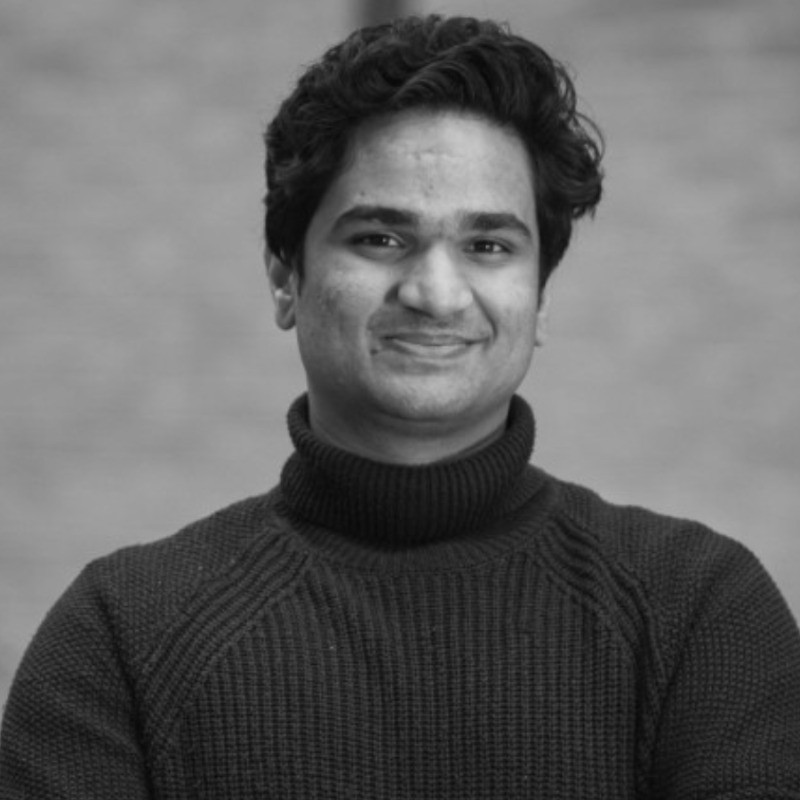
\includegraphics[width=2.0cm]{photo.jpg}
\end{minipage}
\vspace{-2pt}

% ================= SUMMARY =================
\section{Summary}
% >>> TAILOR 2 — SUMMARY: 3-4 lines, plain voice, no em-dashes. Open with the
%     one thing this JD most wants, backed by his real FlowSpace work. Keep to
%     his facts. One-page fit lever #3: trim this to 3 lines if it spills.
I build workflow automations, integrations and AI agents in production, and I ship the full-stack code around them. At FlowSpace I designed and maintained n8n-based CRM and GTM automations connecting multiple systems via APIs and webhooks, built LLM-powered agents that answer customer queries against live data, and built an AI listing pipeline that turns any document format into structured output with a human in the loop. I work across business functions (sales, marketing, customer success, operations) to identify automation opportunities and translate them into technical solutions. I write Python, TypeScript and Node.js, and wire in OpenAI and Claude APIs.

% ================= SKILLS =================
\section{Skills}
% >>> TAILOR 3 — SKILLS: reorder so the FIRST bullet leads with what the JD
%     emphasises (agents / migrations / full-stack / GTM automation ...).
%     One-page fit lever #4: drop the last bullet if the page spills.
\begin{itemize}
 \item \textbf{Automation \& AI:} n8n workflow automation, AI agents built and operated in production, LLM APIs (OpenAI, Claude), RAG, prompt and context engineering, human-in-the-loop review, evals, Microsoft Power Automate certified
 \item \textbf{Languages \& platforms:} Python, TypeScript, JavaScript, Next.js, React, Node.js, Laravel (PHP), SQL, PostgreSQL, Supabase
 \item \textbf{Integrations \& data:} REST APIs, webhooks, event-driven architectures, CRM integrations (Attio, Amplemarket), booking systems (OfficeRnD, Nexudus), Google APIs, Sendgrid
 \item \textbf{Cross-functional:} working with sales, marketing, customer success, finance and operations stakeholders to identify automation and AI opportunities, owning problems end to end
\end{itemize}

% ================= EXPERIENCE =================
% Reorder / re-emphasise the FlowSpace bullets per JD, but keep them factual.
% Keep the role title accurate and NON-"Lead" (e.g. "Full-Stack & AI Engineer").
\section{Experience}

\role{\href{https://flowspace.co}{FlowSpace.co}}{Mar 2024 -- Aug 2026}{Full-Stack \& AI Engineer (Full-time, Freelance)}{London, UK (remote)}
\begin{itemize}
 \item Took over a live marketplace on a legacy stack and worked with the team to migrate it to a coded Next.js and Laravel product, mapping the data model and driving the cutover. Scaled it from 2,000 to 4,500+ users.
 \item Built an AI listing bot with a human in the loop: it takes a brochure in any format (PDF, web page, photo or spreadsheet), drafts the full listing with an LLM, and pushes it to the backend after review.
 \item Built support AI agents that answer customer queries against live platform data and escalate to a person on low confidence.
 \item Built CRM and GTM automations with n8n, including a pipeline connecting Attio, Amplemarket and Swan, plus OfficeRnD and Nexudus booking integrations.
 \item Worked directly with the internal team, an external agency and customers, and resolved issues end to end.
\end{itemize}

\role{\href{https://get2germany.com}{Get2Germany.com}}{Jan 2024 -- May 2024}{Developer \& Automation Specialist (Part-time)}{Berlin, Germany}
Integrated Google APIs, built AI tools to find courses, internships and jobs, and optimized the database. Stack: n8n, Google APIs.\\[1pt]

\role{\href{https://clubee.com}{Clubee.com}}{Sep 2023 -- Aug 2024}{Developer \& QA (Full-time, Freelance)}{Foetz, Luxembourg}
Integrated the Clubee API across the frontend, ran unit testing and QA, and built shop and federation-dashboard tools.\\[1pt]

\role{\href{https://tractionboard.co}{Tractionboard.co}}{Aug 2023 -- Oct 2023}{Developer (Internship)}{Utrecht, Netherlands}
Integrated ChatGPT/OpenAI and Sendgrid, built responsive designs, and debugged features.

% ================= FREELANCE PROJECTS =================
\section{Freelance Projects}
\begin{itemize}
 \item \textbf{\href{https://smarturlink.com/}{Urlink}} (2025), Project Manager \& AI-Assisted Developer. Worked directly with the client on requirements, built the platform and its logic, and implemented client-driven automations. Stack: Next.js, Supabase, Netlify.
 \item \textbf{\href{https://ultrastrategy.com}{UltraStrategy}} (2024 to 2025), AI Automation Developer. Built a CV-parsing tool (LLM data extraction) with n8n and Eden AI, and a platform serving different user profiles.
 \item \textbf{\href{https://www.qomodo.me/}{Qomodo}} (2024 to 2025), AI Developer. Built a dashboard for companies to manage their branches, and implemented Figma designs.
\end{itemize}

% ================= CERTIFICATIONS =================
\section{Certifications}
Microsoft Copilot Studio Agent Academy \textbullet\ Microsoft: Introduction to building AI agents \textbullet\ Microsoft Power Automate \textbullet\ Tray.AI Build Practitioner (Sep 2024)

% ================= EDUCATION =================
\section{Education}
\textbf{Ca' Foscari University of Venice} \hfill Oct 2020 -- Jun 2024\\
BA Philosophy, International Studies \& Economics (Minor: Entrepreneurship)

% ================= AUTH =================
% One-page fit lever #5: \vspace{2pt} here (not 4pt); drop "open to remote" if it spills.
\vspace{2pt}
{\small \textbf{Work authorization:} European Long Term Residence Permit (Italy), no sponsorship needed in the EU; available immediately. \quad \textbf{Languages:} Hindi (native), English (professional), Italian (beginner).}

\end{document}
